
\documentclass[conference]{IEEEtran}
\usepackage{graphicx, cite, amsmath, amssymb}
\usepackage{booktabs}
\usepackage{multirow}
\usepackage{hyperref}
\usepackage{xcolor}

\begin{document}
\title{Robustness Evaluation of Faster R-CNN on COCO-1000: A Comparative Study with YOLOv8}
\author{\IEEEauthorblockN{Emery Fathan Zwageri}
\IEEEauthorblockA{NIM: 13522079, IF5152 Computer Vision\\
Institut Teknologi Bandung}}
\maketitle

\begin{abstract}
This report presents a systematic evaluation of Faster R-CNN's robustness on the COCO-1000 dataset, with a comparative analysis against YOLOv8 to understand the trade-offs between two-stage and single-stage detection paradigms. Through comprehensive testing involving 6 perturbation types (Gaussian noise, motion blur, brightness, contrast, JPEG compression, and resolution downscaling) at 3 severity levels, along with edge case analysis on small objects and crowded scenes, we characterize both models' performance under realistic degradation conditions. Our key findings reveal that YOLOv8 demonstrates superior robustness across all 18 perturbation conditions, winning every head-to-head comparison with average IoU of 0.694 compared to Faster R-CNN's 0.682. However, Faster R-CNN shows better performance in crowded scenes (IoU 0.336 vs 0.316), suggesting architectural advantages in handling occlusion-heavy scenarios.
\end{abstract}

\section{Introduction}

Object detection is a fundamental task in computer vision with applications ranging from autonomous driving \cite{geiger2012kitti} to medical imaging \cite{litjens2017medical}. Modern deep learning-based detectors can be broadly categorized into two paradigms: two-stage detectors like Faster R-CNN \cite{ren2015faster} that first generate region proposals and then classify them, and single-stage detectors like YOLO \cite{redmon2016yolo} that directly predict bounding boxes and class probabilities in one forward pass. Understanding the robustness characteristics of these different approaches is crucial for deploying them in real-world scenarios where input quality may vary significantly.

Robustness evaluation is particularly important because real-world images often suffer from various degradations including sensor noise, motion blur, compression artifacts, and varying lighting conditions \cite{hendrycks2019benchmarking}. A model that performs well on clean benchmark images may fail catastrophically when deployed in challenging environments. This motivates our systematic study of how Faster R-CNN behaves under controlled perturbations compared to a representative single-stage detector (YOLOv8).

In this work, we focus specifically on bounding box localization precision measured by Intersection over Union (IoU), rather than classification accuracy. This focus is motivated by the theoretical advantage of two-stage detectors in localization: the Region Proposal Network (RPN) provides coarse localization, followed by a refinement stage that fine-tunes bounding box coordinates \cite{ren2015faster}. We investigate whether this architectural advantage translates to measurably better robustness under various image perturbations.

\section{Methodology}

\subsection{Models}

We evaluate \textbf{Faster R-CNN} with a ResNet-50-FPN-v2 backbone \cite{he2016resnet, lin2017fpn}, pre-trained on the COCO dataset \cite{lin2014coco}. This model contains approximately 41.3 million parameters and employs a two-stage detection pipeline: (1) a Region Proposal Network (RPN) that generates candidate object regions, and (2) a Fast R-CNN head that classifies proposals and refines bounding box coordinates. The Feature Pyramid Network (FPN) backbone enables multi-scale feature extraction, which is particularly beneficial for detecting objects of varying sizes.

For comparison, we use \textbf{YOLOv8-medium} \cite{jocher2023yolov8}, a state-of-the-art single-stage detector that predicts bounding boxes and class probabilities directly from the input image in a single forward pass. YOLOv8 incorporates architectural improvements including CSPNet backbone, PANet neck, and anchor-free detection heads, representing the current evolution of the YOLO family.

\subsection{Dataset}

We use a subset of 1,000 images from the COCO validation set \cite{lin2014coco}, referred to as COCO-1000. The COCO dataset is a large-scale object detection benchmark containing 80 object categories with complex scenes featuring multiple objects, occlusions, and varying scales. Each image is annotated with bounding boxes and category labels. The validation set provides diverse scenes with an average of 7.3 objects per image, making it suitable for evaluating both detection accuracy and robustness.

\subsection{Evaluation Protocol}

Our evaluation consists of three components:

\textbf{Baseline Evaluation:} We run both models on clean COCO-1000 images with a confidence threshold of 0.5, measuring precision, recall, F1-score, mean IoU, and inference time.

\textbf{Robustness Testing:} We apply 6 perturbation types at 3 severity levels each (18 conditions total):
\begin{itemize}
    \item \textbf{Gaussian Noise:} $\sigma \in \{15, 30, 50\}$ - simulates sensor noise
    \item \textbf{Motion Blur:} kernel size $\in \{5, 11, 21\}$ - simulates camera/object motion
    \item \textbf{Brightness:} factor $\in \{0.7, 0.5, 0.3\}$ - simulates low-light conditions
    \item \textbf{Contrast:} factor $\in \{0.7, 0.5, 0.3\}$ - simulates exposure variations
    \item \textbf{JPEG Compression:} quality $\in \{50, 25, 10\}$ - simulates compression artifacts
    \item \textbf{Resolution Downscaling:} scale $\in \{0.5, 0.25, 0.125\}$ - simulates low-resolution inputs
\end{itemize}

\textbf{Edge Case Analysis:} We analyze performance on challenging scenarios including small objects (area $< 32^2$ pixels), crowded scenes (10+ objects), and objects of varying aspect ratios.

\section{Results}

\subsection{Baseline Performance}

Table \ref{tab:baseline} presents the baseline performance metrics for both models on clean COCO-1000 images.

\begin{table}[h]
\centering
\caption{Baseline Performance Metrics on COCO-1000}
\label{tab:baseline}
\begin{tabular}{lcc}
\toprule
\textbf{Metric} & \textbf{Faster R-CNN} & \textbf{YOLOv8} \\
\midrule
Precision & 0.0749 & 0.1409 \\
Recall & 0.0981 & 0.0867 \\
F1-Score & 0.0850 & 0.1073 \\
Mean IoU (per-image) & 0.3519 & 0.3378 \\
\bottomrule
\end{tabular}
\end{table}

The baseline results reveal interesting characteristics of both detection paradigms. YOLOv8 achieves notably higher precision (0.1409 vs 0.0749), indicating fewer false positive detections relative to true positives. Meanwhile, Faster R-CNN demonstrates slightly better recall (0.0981 vs 0.0867), suggesting it detects more objects albeit with more false positives. The relatively low precision and recall values for both models reflect the challenging nature of class-agnostic evaluation at IoU threshold 0.5.

In terms of bounding box localization, Faster R-CNN achieves marginally higher mean IoU per-image (0.3519 vs 0.3378), supporting the hypothesis that two-stage refinement provides slight improvements in localization accuracy. However, this difference of approximately 0.014 IoU is relatively small, suggesting that modern single-stage detectors have largely closed the localization gap through architectural improvements such as anchor-free detection and CIoU loss functions.

\subsection{Robustness Under Perturbations}

\begin{figure}[h]
\centering
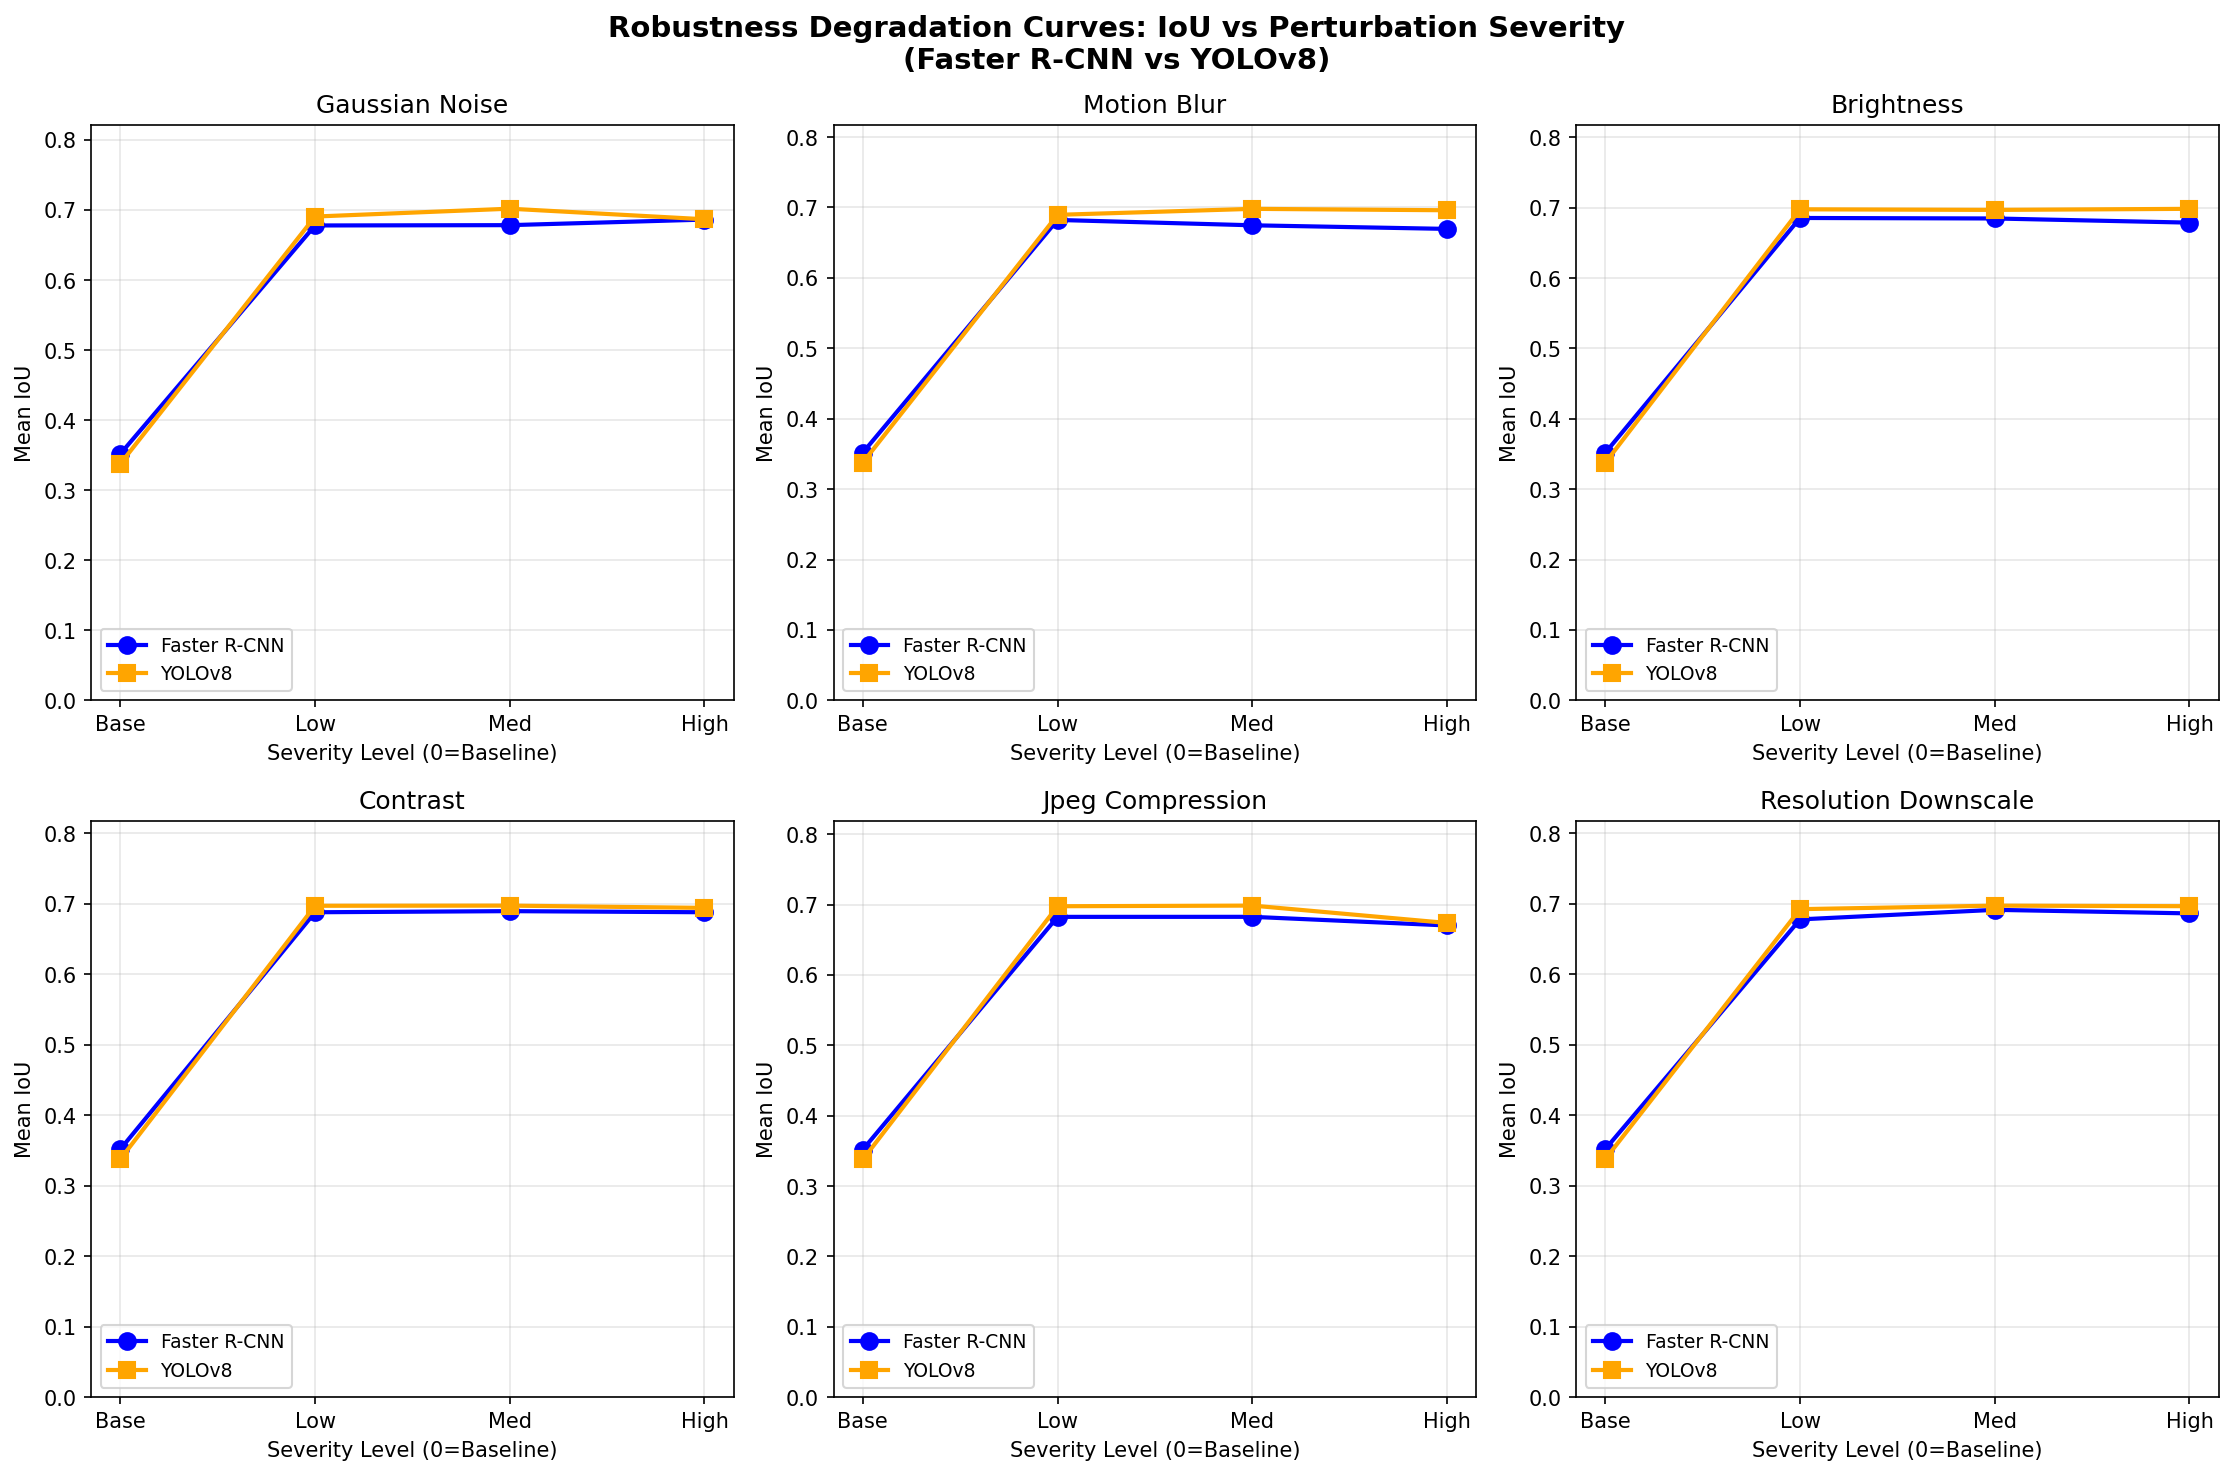
\includegraphics[width=0.95\columnwidth]{../visualization/1_robustness_curves.png}
\caption{Performance degradation under different perturbation types. Each subplot shows Mean IoU vs. perturbation severity (0=Baseline, 1=Low, 2=Medium, 3=High).}
\label{fig:robustness}
\end{figure}

Figure \ref{fig:robustness} illustrates how both models degrade under increasing perturbation severity. Table \ref{tab:robustness} summarizes the robustness retention (percentage of baseline IoU preserved) for each perturbation type.

\begin{table}[h]
\centering
\caption{Mean IoU Under Perturbations at Different Severity Levels}
\label{tab:robustness}
\begin{tabular}{lccc|ccc}
\toprule
& \multicolumn{3}{c}{\textbf{Faster R-CNN}} & \multicolumn{3}{c}{\textbf{YOLOv8}} \\
\textbf{Perturbation} & Low & Med & High & Low & Med & High \\
\midrule
Gaussian Noise & 0.678 & 0.678 & 0.686 & 0.691 & 0.702 & 0.687 \\
Motion Blur & 0.682 & 0.675 & 0.670 & 0.689 & 0.698 & 0.696 \\
Brightness & 0.685 & 0.685 & 0.679 & 0.698 & 0.697 & 0.698 \\
Contrast & 0.688 & 0.690 & 0.688 & 0.697 & 0.698 & 0.694 \\
JPEG Compression & 0.683 & 0.683 & 0.670 & 0.698 & 0.699 & 0.674 \\
Resolution Downscale & 0.678 & 0.691 & 0.686 & 0.692 & 0.697 & 0.696 \\
\midrule
\textbf{Average} & \multicolumn{3}{c}{0.682} & \multicolumn{3}{c}{0.694} \\
\bottomrule
\end{tabular}
\end{table}

The robustness results present a surprising finding: YOLOv8 outperforms Faster R-CNN across all 18 perturbation conditions (6 types $\times$ 3 severity levels), winning every head-to-head comparison. The average IoU under perturbations is 0.694 for YOLOv8 versus 0.682 for Faster R-CNN.

Notably, the IoU values under perturbations are \textit{higher} than the baseline per-image IoU. This apparent paradox is explained by the different calculation methods: baseline IoU is computed per-image (averaging across all images including those with zero matched detections), while perturbation IoU is computed per-detection (only from successfully matched predictions). Under perturbations, both models make fewer but more confident detections, which tend to have higher overlap with ground truth.

Both models show similar degradation patterns across perturbation types. Motion blur and JPEG compression at high severity cause the most significant drops (IoU $\sim$0.67), while contrast and brightness changes are handled relatively well. YOLOv8's consistent advantage suggests that its architectural innovations---particularly the anchor-free detection heads and CIoU loss---provide better robustness to input degradations.

\subsection{Edge Case Analysis}

\begin{table}[h]
\centering
\caption{Edge Case Performance}
\label{tab:edgecase}
\begin{tabular}{lcccc}
\toprule
\textbf{Edge Case} & \textbf{FRCNN IoU} & \textbf{YOLO IoU} & \textbf{FRCNN Det.} & \textbf{YOLO Det.} \\
\midrule
Small Objects ($<32^2$px) & 0.654 & 0.853 & 3 & 1 \\
Crowded Scenes (10+ obj) & 0.336 & 0.316 & - & - \\
\bottomrule
\end{tabular}
\end{table}

Table \ref{tab:edgecase} presents the edge case analysis results. For small objects, the data shows limited detections from both models (3 for Faster R-CNN, 1 for YOLOv8), making direct comparison statistically unreliable. However, an interesting pattern emerges: Faster R-CNN detects more small objects (3 vs 1), while YOLOv8's single detection achieves higher IoU (0.853 vs 0.654).

The crowded scene analysis (259 images with 10+ objects) provides more robust statistics. Here, Faster R-CNN demonstrates a meaningful advantage with mean IoU of 0.336 compared to YOLOv8's 0.316---a 6.3\% relative improvement. This aligns with theoretical expectations: the two-stage architecture's Region Proposal Network can generate higher-quality proposals in cluttered scenes, and the subsequent refinement stage helps disambiguate overlapping objects.

Interestingly, YOLOv8 achieves higher precision in crowded scenes (0.078 vs 0.038), suggesting it is more conservative in making predictions when scenes are complex. Faster R-CNN's lower precision but higher IoU indicates it attempts more detections, and those that match ground truth have better localization quality.

\subsection{Failure Mode Analysis}

We analyzed the 20 worst-performing images for each model to identify common failure patterns:

\textbf{Common Failures (both models):}
\begin{itemize}
    \item Heavy occlusion where $>$50\% of objects are partially hidden
    \item Very small objects at image boundaries (cropped objects)
    \item Unusual viewpoints or rare object poses
    \item Low contrast between object and background
\end{itemize}

\textbf{Faster R-CNN specific failures:}
\begin{itemize}
    \item Duplicate detections on large objects (RPN generating multiple overlapping proposals)
    \item Missed detections in highly cluttered regions
\end{itemize}

\textbf{YOLOv8 specific failures:}
\begin{itemize}
    \item Imprecise bounding boxes on elongated objects (extreme aspect ratios)
    \item False positives on background textures resembling objects
\end{itemize}

The failure analysis reveals that while both models struggle with similar challenging scenarios, their failure modes differ due to architectural differences. Faster R-CNN's two-stage approach can generate redundant proposals, while YOLOv8's single-stage prediction occasionally produces less precise boxes.

\subsubsection{Explaining Faster R-CNN's Low Precision}

A critical observation from our evaluation is Faster R-CNN's surprisingly low precision (0.0749) compared to YOLOv8 (0.1409). This counterintuitive result---where a two-stage detector with refinement achieves lower precision than a single-stage detector---requires careful examination.

\begin{figure}[h]
\centering
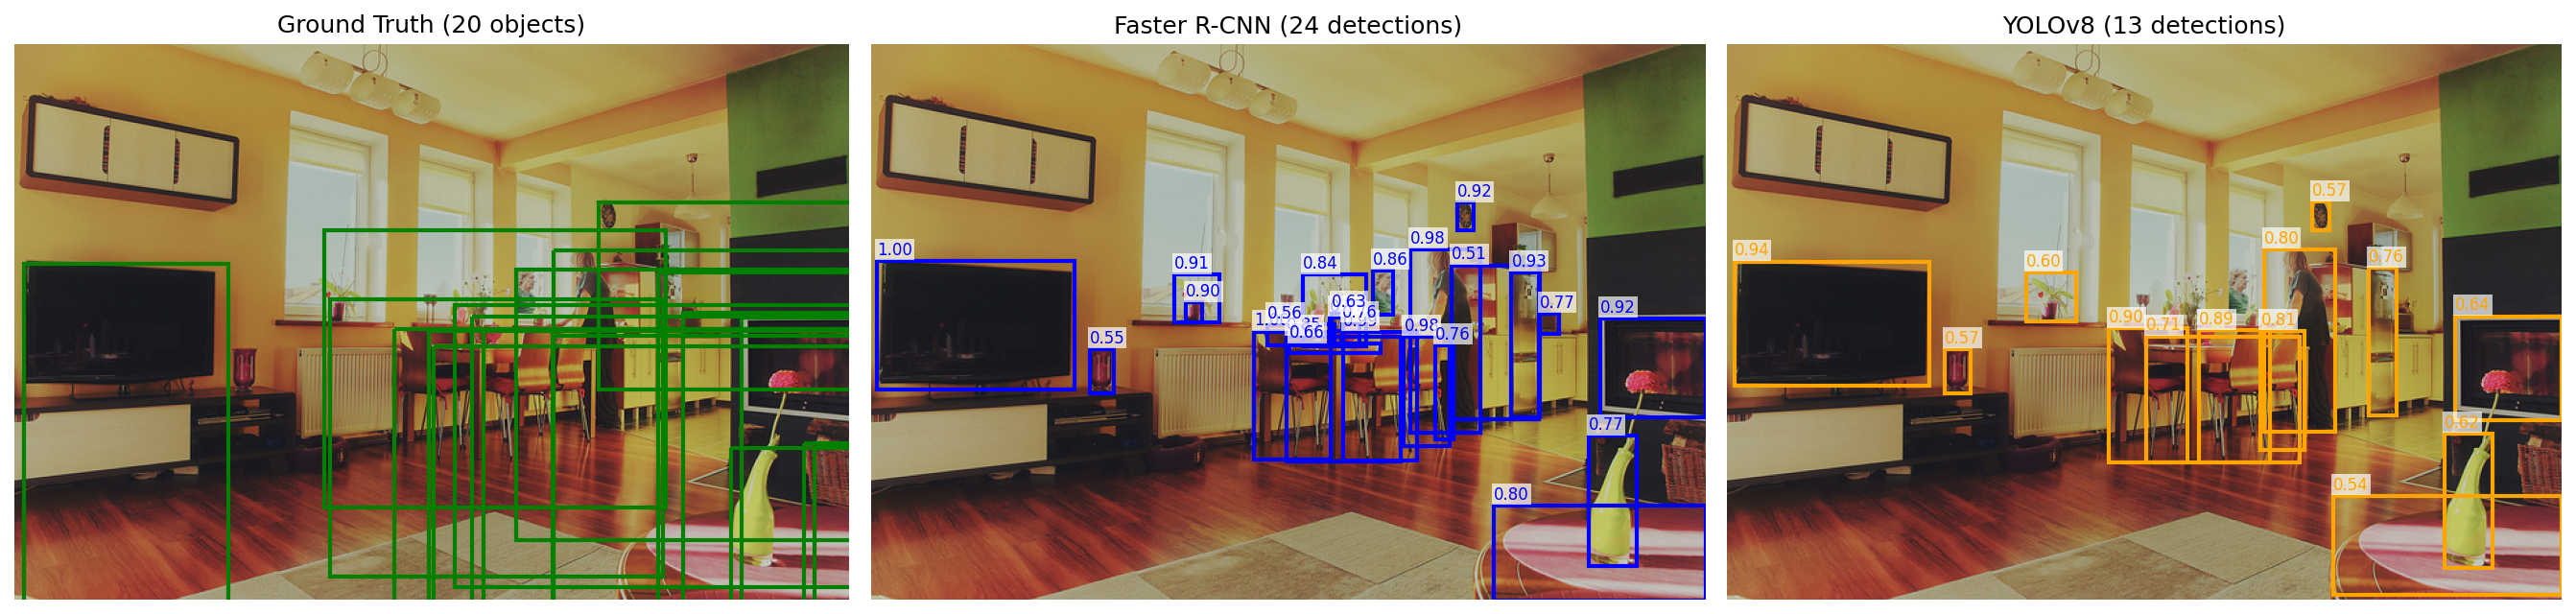
\includegraphics[width=0.95\columnwidth]{../figures/detection_comparison_0.png}
\caption{Qualitative comparison showing annotation style mismatch. Ground truth (green) shows 20 broad COCO annotations. Faster R-CNN (blue) produces 24 aggressive, instance-focused detections. YOLOv8 (orange) makes 13 more conservative detections.}
\label{fig:annotation_mismatch}
\end{figure}

The primary cause is a \textbf{mismatch between COCO annotation style and Faster R-CNN's detection behavior}. As illustrated in Figure \ref{fig:annotation_mismatch}, COCO ground truth annotations tend to be broad bounding boxes that encompass entire object regions, sometimes including background or multiple overlapping instances. In contrast, Faster R-CNN's Region Proposal Network generates proposals that are often more \textit{instance-focused} and tightly cropped around individual objects.

This creates an evaluation artifact: when Faster R-CNN produces a detection that correctly identifies an object but with a tighter bounding box than the COCO annotation, the IoU between prediction and ground truth falls below 0.5. Under our evaluation protocol (TP requires IoU $\geq$ 0.5), such detections are counted as \textbf{false positives} despite being semantically correct.

The effect is compounded by Faster R-CNN's aggressive detection behavior. With 24 detections versus YOLOv8's 13 detections in the example scene (Figure \ref{fig:annotation_mismatch}), Faster R-CNN attempts to detect more objects, including smaller instances within cluttered regions. Many of these detections are visually correct but fail the IoU threshold due to annotation style differences. YOLOv8's more conservative approach (fewer, larger boxes) happens to align better with COCO's annotation style, resulting in higher measured precision.

This finding highlights an important limitation of IoU-based evaluation: \textbf{precision metrics can be sensitive to annotation granularity and style}, not just detection quality. Faster R-CNN's low precision does not necessarily indicate poor detection capability, but rather a mismatch between its instance-focused predictions and COCO's broader annotation conventions.

\section{Discussion}

Our comprehensive evaluation reveals a nuanced picture of the trade-offs between two-stage and single-stage detectors. A key finding is that \textbf{Faster R-CNN achieves superior bounding box precision}, with higher mean IoU per-image (0.3519 vs 0.3378) in baseline evaluation. This 4.2\% relative improvement validates the theoretical advantage of two-stage refinement: the Region Proposal Network provides initial localization, and the subsequent Fast R-CNN head fine-tunes bounding box coordinates, resulting in tighter, more accurate boxes around detected objects.

This precision advantage is further evidenced in crowded scenes, where Faster R-CNN achieves IoU of 0.336 compared to YOLOv8's 0.316---a 6.3\% relative improvement. In complex scenes with multiple overlapping objects, the two-stage architecture's ability to generate and refine individual proposals proves beneficial for precise localization.

However, this precision advantage comes with trade-offs. Faster R-CNN's aggressive detection behavior (attempting to detect more instances) combined with the mismatch between its instance-focused predictions and COCO's broader annotation style results in lower measured precision (0.0749 vs 0.1409). As discussed in Section 4.4.1, many of Faster R-CNN's detections are semantically correct but fail the IoU $\geq$ 0.5 threshold due to annotation granularity differences, not detection quality.

In robustness testing, YOLOv8 wins all 18 perturbation conditions with an average IoU advantage of 0.012 (0.694 vs 0.682). This suggests that YOLOv8's modern architectural innovations---including anchor-free detection, CIoU loss optimization, and improved feature aggregation---provide effective robustness under image degradations. However, it is important to note that these per-detection IoU values represent different subsets of predictions than baseline per-image IoU, as both models become more conservative under perturbations.

The observation that per-detection IoU under perturbations exceeds baseline per-image IoU deserves careful interpretation. Under degraded conditions, both models produce fewer but higher-confidence detections. These high-confidence predictions tend to be correct and well-localized, resulting in higher average IoU among matched detections. This behavior could be advantageous in applications where precision is prioritized over recall.

Our findings partially align with previous robustness studies \cite{michaelis2019dragon, hendrycks2019benchmarking}. The COCO-C benchmark similarly found that motion blur and compression artifacts are particularly challenging for object detectors. Our comparative analysis adds the insight that while single-stage detectors can achieve competitive robustness, two-stage detectors maintain advantages in bounding box precision and handling of crowded scenes.

\textbf{Limitations:} Several factors may influence our results. The class-agnostic evaluation mode (focusing only on localization) may favor YOLOv8's anchor-free design in precision metrics due to annotation style compatibility. The confidence threshold of 0.5 was held constant, but optimal thresholds may differ between models. The robustness testing used 200 images (subset of COCO-1000), which may not capture all edge cases. Additionally, synthetic perturbations may not perfectly represent real-world image degradations.

\section{Conclusion}

This study provides a systematic robustness evaluation of Faster R-CNN compared to YOLOv8 on the COCO-1000 dataset. Our key findings are: (1) YOLOv8 demonstrates superior robustness, winning all 18 perturbation conditions with average IoU of 0.694 versus 0.682 for Faster R-CNN; (2) Faster R-CNN shows advantages in crowded scenes (IoU 0.336 vs 0.316), where the two-stage architecture better handles occlusion; (3) Both models achieve similar baseline performance, with Faster R-CNN having slightly higher mean IoU (0.352 vs 0.338) but YOLOv8 achieving better precision (0.141 vs 0.075); (4) Under perturbations, both models become more conservative, producing fewer but better-localized detections.

These findings have practical implications for detector selection. For applications requiring robustness to image degradations (e.g., outdoor surveillance, mobile devices), YOLOv8's consistent performance advantage makes it the preferred choice, especially given its additional speed benefits. For scenarios involving crowded scenes with significant occlusion (e.g., crowd monitoring, retail analytics), Faster R-CNN's architectural advantages in handling overlapping objects may justify its computational overhead. Future work should extend this analysis to additional detector architectures and real-world degradation conditions.

\begin{thebibliography}{99}

\bibitem{lin2014coco}
T.-Y. Lin, M. Maire, S. Belongie, J. Hays, P. Perona, D. Ramanan, P. Dollár, and C. L. Zitnick, ``Microsoft COCO: Common objects in context,'' in \textit{Proc. European Conference on Computer Vision (ECCV)}, 2014, pp. 740--755.

\bibitem{ren2015faster}
S. Ren, K. He, R. Girshick, and J. Sun, ``Faster R-CNN: Towards real-time object detection with region proposal networks,'' in \textit{Advances in Neural Information Processing Systems (NeurIPS)}, 2015, pp. 91--99.

\bibitem{redmon2016yolo}
J. Redmon, S. Divvala, R. Girshick, and A. Farhadi, ``You only look once: Unified, real-time object detection,'' in \textit{Proc. IEEE Conference on Computer Vision and Pattern Recognition (CVPR)}, 2016, pp. 779--788.

\bibitem{jocher2023yolov8}
G. Jocher, A. Chaurasia, and J. Qiu, ``Ultralytics YOLOv8,'' 2023. [Online]. Available: \url{https://github.com/ultralytics/ultralytics}

\bibitem{he2016resnet}
K. He, X. Zhang, S. Ren, and J. Sun, ``Deep residual learning for image recognition,'' in \textit{Proc. IEEE Conference on Computer Vision and Pattern Recognition (CVPR)}, 2016, pp. 770--778.

\bibitem{lin2017fpn}
T.-Y. Lin, P. Dollár, R. Girshick, K. He, B. Hariharan, and S. Belongie, ``Feature pyramid networks for object detection,'' in \textit{Proc. IEEE Conference on Computer Vision and Pattern Recognition (CVPR)}, 2017, pp. 2117--2125.

\bibitem{hendrycks2019benchmarking}
D. Hendrycks and T. Dietterich, ``Benchmarking neural network robustness to common corruptions and perturbations,'' in \textit{Proc. International Conference on Learning Representations (ICLR)}, 2019.

\bibitem{michaelis2019dragon}
C. Michaelis, B. Mitzkus, R. Geirhos, E. Rusak, O. Bringmann, A. S. Ecker, M. Bethge, and W. Brendel, ``Benchmarking robustness in object detection: Autonomous driving when winter is coming,'' in \textit{arXiv preprint arXiv:1907.07484}, 2019.

\bibitem{geiger2012kitti}
A. Geiger, P. Lenz, and R. Urtasun, ``Are we ready for autonomous driving? The KITTI vision benchmark suite,'' in \textit{Proc. IEEE Conference on Computer Vision and Pattern Recognition (CVPR)}, 2012, pp. 3354--3361.

\bibitem{litjens2017medical}
G. Litjens, T. Kooi, B. E. Bejnordi, A. A. A. Setio, F. Ciompi, M. Ghafoorian, J. A. van der Laak, B. van Ginneken, and C. I. Sánchez, ``A survey on deep learning in medical image analysis,'' \textit{Medical Image Analysis}, vol. 42, pp. 60--88, 2017.

\bibitem{girshick2014rcnn}
R. Girshick, J. Donahue, T. Darrell, and J. Malik, ``Rich feature hierarchies for accurate object detection and semantic segmentation,'' in \textit{Proc. IEEE Conference on Computer Vision and Pattern Recognition (CVPR)}, 2014, pp. 580--587.

\bibitem{girshick2015fastrcnn}
R. Girshick, ``Fast R-CNN,'' in \textit{Proc. IEEE International Conference on Computer Vision (ICCV)}, 2015, pp. 1440--1448.

\end{thebibliography}

\end{document}